% EPL master thesis cover template
\documentclass{eplmastersthesis}

% help package for todo
\usepackage{xargs}                      % Use more than one optional parameter in a new commands
\usepackage[pdftex,dvipsnames]{xcolor}  % Coloured text etc.
% 
\usepackage{hyperref} % for url and so on
\usepackage[colorinlistoftodos,prependcaption,textsize=tiny]{todonotes}
\newcommandx{\unsure}[2][1=]{\todo[linecolor=red,backgroundcolor=red!25,bordercolor=red,#1]{#2}}
\newcommandx{\change}[2][1=]{\todo[linecolor=blue,backgroundcolor=blue!25,bordercolor=blue,#1]{#2}}
\newcommandx{\info}[2][1=]{\todo[linecolor=OliveGreen,backgroundcolor=OliveGreen!25,bordercolor=OliveGreen,#1]{#2}}
\newcommandx{\improvement}[2][1=]{\todo[linecolor=Plum,backgroundcolor=Plum!25,bordercolor=Plum,#1]{#2}}
\newcommandx{\thiswillnotshow}[2][1=]{\todo[disable,#1]{#2}}

% Fill in here the information: title, student name, speciality, jury members
\title{Privacy Aware Sharing of IOCs in MISP}	% Master thesis title
%\subtitle{Subtitle (optional)}			% Optional subtitle
\author{Charles \textsc{Jacquet}}	% Student name
%\secondauthor{Firstname \textsc{Lastname}}	% Second student name if applicable
\speciality{Computer Science and Engineering}		% Speciality (use one of the following options):
										% Biomedical Engineering
										% Chemical and Materials Engineering
										% Civil Engineering
										% Computer Science
										% Computer Science and Engineering
										% Electrical Engineering
										% Electro-mechanical Engineering
										% Mathematical Engineering
										% Mechanical Engineering
										% Physical Engineering
%\options{Option(s)}		% If required by program commission mention options
\supervisor{Ramin \textsc{Sadre}}	% 1st supervisor name
%\cosupervisor{Firstname \textsc{Lastname}}	% 2nd supervisor name if applicable
\readerone{Antoine \textsc{Cailliau}, Alexandre \textsc{Dulaunoy}}		% 1st reader name
\readertwo{William \textsc{Robinet}}		% 2nd reader name
\readerthree{François-Xavier \textsc{Standaert}}	% 3rd reader name
\years{2016-2017}	% Academic year

\begin{document}

\maketitle					% To create front cover page
\thispagestyle{empty}		% To suppress header and footer on the back of the cover page


\begin{abstract} 
Malicious software (malware) are plaguing this computer age. But how to avoid them ?
An actual solution is threat information sharing where companies share lists of Indicators Of Compromise (e.g. IPs, mail addresses, urls, malware hashes and so on) with each other.
An interesting tool is the MISP (Malware Information Sharing Platform), a platform that allows companies to share these IOCs but also malware analysis.
Sometimes, the information is somehow confidential, but still interesting to be shared, thus we need to find a way to share these secret information without disclosing them entirely.
The goal of this master thesis will be to analyze the state of the art and to implement different solutions working with MISP in order to compare their performances.
\end{abstract}

\tableofcontents

\chapter{Introduction}
\section{Interaction with this Latex Document (To be removed)}
In order to facilitate comments, I've added some new commands explained by\footnote{http://tex.stackexchange.com/questions/9796/how-to-add-todo-notes}:\\
\begin{itemize}
\item unsure => What I need to check
\item change => What have to be modified
\item info => Add simple comment
\item improvement => Indicate a possible improvement
\end{itemize}

\section{Introduction}
In the last report of the Ponemon institute, we can see that the estimated cost of annual data breaches for 384 companies in 12 countries\footnote{United States, United Kingdom, Germany, Australia, France, Brazil, Japan, Italy, India, the Arabian region (United Arab Emirates and Saudi Arabia), Canada and, South Africa} is about \$4 million. Moreover, 48\% of theses breaches are due to malicious and criminal attacks.\\
Taking that into account, the damage cost per capita is about \$170 only for malicious and criminal attacks. \\
Beside that, Cybersecurity Ventures predicts the global annual cybercrime costs will grow from \$3 trillion in 2015 to 6\$ trillion by 2021.\\

We thus need to improve our computer defenses and make them to learn continuously about new appearing threats. Moreover, they should be aware of new threats faster than simple malware detectors or anti-viruses. This is why a new kind of security levels appeared and is called threat sharing. As soon as an organization find a malware, they can prevent others to be compromised just by letting them know about the threat. \\
Unfortunately, this is not enough as, theses informations, here and after called IOCs, are often considered as confidential because revealing them, can reveal damaging information for the companies.\\
We thus need to find a way for \textbf{sharing} information without \textbf{giving} the information. And I will try to explain the meaning of this sentence in the report's body. But, for now, we can say that this master's thesis is on finding a "more secure" way of sharing information. More precisely, if we attempt to create an encrypted database of these IOCs, the idea would be to slow down as much as possible a brute force attack for someone who has complete access to the database while still making this database useful for the targeted user.\\

I've decided to organize the work the same way I've discovered and implemented things but I'm firstly defining the tools an vocabulary that will be used. I'll be continuing this chapter with a state of the art that made me understood the domain and the limitation that I was going to face.\\
Afterwards, I'll spoke about the implementation ideas I've got, by highlighting theirs strengths and weaknesses. While the third chapter will really be about my implementations, my choices on the system but not only on the way I've implement things but also the library I've chosen.\\
The next one will be an analyze of the implementation supported with different benchmarks.\\
Finally, I will conclude on my work with some possible improvement and future work but also by concluding on every thing I've discovered.

\section{Organization}
Before going down in the subject, I also think that it is interesting to point out some aspects of the way I've worked on this project.\\
Firstly, last year, I was searching for a security subject but unfortunately, I wasn't really excited about the proposed ones. But in the other side, I had no idea either on what I could work. I had just the idea to specialize myself into cyber security. Thus, I've looked for ideas where there are plenty of them, directly in security companies.\\
I've found a company called Conostix which provides security and system services in Luxembourg.\\
They weren't short of ideas, and even if I have to admit that I didn't understand everything, it seemed really interesting. Later on, William Robinet (from conostix) contacted me again to say that they have a better idea and it was to work on MISP. I've thus met Alexandre Dulaunoy from CIRCL and they gave me the starting point of the project which was malware sharing in MISP.\\

As I had zero knowledge in this domain, I've chosen to make an internship of four weeks in the company (with no course credits) where I've learned the basics of MISP and I've also worked on network log parsing. But what I mostly learned was that four weeks for trying to specialize myself in a completely new domain wasn't enough but just gave me a rough idea of what it is.\\
During these four weeks, I mostly worked on logs. I've created nothing new, actually it was quite the opposite but it was still interesting to understand how things were working and why they could be useful. \\
In short, during this internship, I've started to understand how squid3 was working. Then I've installed it on my computer in order to get logs to work on.\\
Once I've my logs, I would like to get information from them, thus, I've tried to manually parse the logs (which was a mistake). For that purpose, I've started to implement a parser that was using regex to transform each log lines into a set of objects. But even if it was funny to implement, I spent a lot of time on it and each time I finished, I found it not good enough, not modular enough, losing locality and ordering information, and so on. I have thus realized that I was loosing my time as, of course they are plenty of tools for this kind of job like Logstash.\\
Then I've started to work with MISP to see how it was working. I've reimplemented a similar hash store like the misp-workbench project.\\
I've then used it with my log system by parsing the data from MISP the same way I was parsing the logs before adding them to the hash database on Redis.\\
(Redis was also a great tool I've learned about and that I think that the time I spent on it worth it.)\\
I've then created a system to feed the parsed log in my system and briefly analyze the logs.\\
Beside that, I also had the opportunity to benefit from a one day MISP training organized by CIRCL.
I have then continued to work on my master's thesis the whole year long while keeping in touch with Conostix and CIRCL.

\section{Indicator of Compromise (IOC)}
If there is a crime, detectives can come and look for clues. And they do that because they are wondering questions like what make it happened, why did it happened and how did it happened. The what and why questions can be interesting in order to avoid this crime to happen again while the last one but not the least one, the how can be used to compare this crime with other similar ones.\\
This idea of being able to compare them is really interesting as seeing the clues of only one place can be not enough while there could be enough of them if we succeed in gathering the whole clues of all related crime.\\
This is exactly the same idea here, even if the attacker try to minimize its traces, there are always some. They can be email addresses, IP addresses, malware, url and so on.\\
The idea, is then to use these traces to trigger alarms on other computer system as soon as they are seen. This means that the same attack is perhaps happening again, this is the reason why we call them Indicator Of Compromise.


\section{MISP and Threat Sharing}
I've introduce the idea of malware sharing to defend our computer systems against digital threats and attacks. But MISP is not the only platform to do so, the more current onces are DShield, Critical Stack’s Intel, Microsoft’s Interflow, AlienVault’s Open Threat Exchange, ...\\
But here I focused on the MISP project which is, as said on their website, an open source software solution for collecting, storing, distributing and sharing cyber security indicators and threat about cyber security incidents analysis and malware analysis. MISP is designed by and for incident analysts, security and IT professionals or malware reverser to support their day-to-day operations to share structured informations efficiently.\\
MISP also rely on an hub and spoke sharing model (TAXII \cite{taxiiWebsite}). There is a central point called the hub which is the server where all data are kept and the spokes are the organizations that interact with the hub.\\
A recent paper on MISP \cite{wagner2016misp} had been published this year and could be interesting if your are searching to have a better understanding of the underlying system. Additionally, there is also a recent ietf draft on MISP core format\cite{MispDraft}.\\
I want also to point out that MISP is spreading, and I've the feeling that communities will continue to grow. I've discussed in Belgium with companies like banks, insurances, consultancy companies that are using it which is, at least to my point of view, a good sign on the usage of the system.

\subsection{History}
Christophe Vandeplas started the project as he was tired of the way IOCs were shared (email, pdf, ... ). Thus, he created a cakePHP website as a proof of concept and managed to convince the Belgian Defense (where he was working) that the project was worth to work on. They even allowed him to work on it during his work-hours. The project continued to move forward and now, Andras Iklody is the lead developer of the MISP project and works for CIRCL.\\

\subsection{Basics of Misp}
The basic idea of misp was thus to create an IOC database, for example, if we have two IOCs for the same attack, let's say "IOC@malware.mail" and "192.168.16.2". We are interested to  keep the information that there has been an attack that can be recognized thanks to these two IOCs. That is why they have created events (which is much more general than the term attack that I've been using) and they use these IOCs as the attributes of this specific event. \\
Then thanks to this idea, we can analyze the event and even make correlations with other events if they possess similar IOCs.

For clarity concerns, attributes are divided into 13 categories where they are again dived into types. As MISP is no more only targeting malwares, it is interesting to notice that we can also see categories like Financial Fraud. More standard ones are Network Activities, Antivirus detection, Artifacts dropped, and so on.\\
All the category and types can be found on this web pages \url{https://www.circl.lu/doc/misp/categories-and-types/index.html}

One other really interesting feature is sightings. When an IOC is referenced, we know that it has been seen by someone, but it does not confirm that the IOC is really related to that particular event and is not an error. Moreover, what says that if an IP address is an IOC today that it is going to be the case in 3 months ? \\
Sightings is thus the solution to this problem as we can monitor an IOC, knowing if it has been seen at other places, and if they are still relevant.


There are also two important things on the sharing strategy that I want to point out that are the MISP instances and communities. The first one is easy to understand, MISP is an open source project which means that everybody can decide to run a completely isolated MISP instance for its own needs like a company for storing its own confidential data. Besides that, that does not mean that the instance must be isolated, they have implemented a way to share information between these instances. While the second one is a good property of an instance. When we are connected to MISP as a user, we are connected thanks to the organization that we belongs. Then, the organization can choose to share or not to share their events/attributes with other communities or even with other instances. \\ 

Now, as a good open source project, a whole ecosystem has been created around and more and more companies are using it.\\
MISP become a really good IOC database with automated correlation system. We can even create correlation graphs to see how different events are connected together what helps a lot for the threat analyses.\\
Beside all that, a lot of different tools like a python client library are available on their repository : \url{https://github.com/MISP/}.\\
They have also improved added a lot of value to the web api like the ability of exporting the attributes in a lot of different format and some that can directly be used in IDS.\\

\subsection{My Settings}

There is thus a lot of things to understand in order to work with misp. That's why they are giving trainings and that they make available a misp training virtual machine in order to train ourselves and test new developments.\\
At the beginning, I've started to work directly with the private instance of MISP hosted by CIRCL but, every time that I was working, I needed to have a really good web connection to connect myself and to download all the data. That's why, I have finished by downloading the virtual machine. But, as I was going to work on my computer and I didn't want to be stuck to work inside the virtual machine, I've done some modifications.\\
The mysql database wasn't accessible from the outside of the virtual machine (which is completely understandable as they don't want anyone to have a direct access to the complete unprotected database) and I've also got some network problems.\\
The first step was that my virtual machine running on virtualbox was using the virtual vboxnet0 interface and was using, as its IPv4 address, 192.168.56.50. The problem was that, normally it works without problems but my computer does not know about the subnetwork. I thus had to add an ip in the right range by using the command :
\textbf{ip add add 192.169.56.2/24 dev vboxnet0} .\\
I'm also sometimes using a second virtual machine to work with and on this virtual machine, I've configured two network interfaces, the first one was to have an internet connection while the second one was the vboxnet0 interface.\\
For simplifying the use of the vbox interface, I've configured my network to automatically add an ip in the right range (/etc/network/interfaces). This is the addition on the basic configuration:
\begin{verbatim}
auto eth1
iface eth1 inet static
address 192.168.56.1
netmask 255.255.255.0
\end{verbatim}
 
After that, I was able to contact the virtual machine via the network but it wasn't enough to have a mysql access. For that, as the misp virtal machine was only accessible from the vboxnet0 interface, it was a problem to create external access for all ip addresses with only a small password protection.\\
The first step for that was to modify the configuration file (/etc/mysql/my.conf) where I've juste commented the "bind-address 127.0.0.1" line.
The next step was to create a user with the rights from the outside. For that, I've connected myself to the database as the misp user and I've added the user:
\begin{itemize}
\item[•] mysql -uroot -pPassword1234 
\item[•] CREATE USER 'username'@'\%';
\item[•] GRANT ALL ON *.* TO 'username'@'\%';
\end{itemize}

Once done, I could continue to program more easily and create some tests as I could control the whole available set of data. For testing when the code was modified, I had used a really small set of data. \\
But speaking about testing, I didn't do any automated test as the system requests some connections, It was not easy to generate them. \improvement{Do automated test !}

\subsection{Illustrations}
There is nothing better to explain all that than real screen shot of the web application. But, it raised one really important question: what can and cannot be shared from MISP and with who?\\
For example, Am I allowed to show screen shot of data from MISP without any risk ?\\
To respond to that question, I need to introduce the Traffic Light Protocol (TLP) that was created in order to facilitate information sharing by defining the authorized level of disclosure. And thus, it can be used to know what can be shared with a specific audience.\\
This protocol is defined by FIRST in \cite{FirstTLP} but also in this NIST cyber threat information sharing guide \cite{johnson2016guide}.\\

Knowing that, I know that I can share the data from the virtual machine that I have explained in the previous section as the default OSINT feed is TLP:WHITE. Which means, according to FIRST, that the disclosure is not limited: \\
Sources may use TLP:WHITE when information carries minimal or no foreseeable risk of misuse, in accordance with applicable rules and procedures for public release. Subject to standard copyright rules, TLP:WHITE information may be distributed without restriction.\\

The first pages (after the connection) of the web application is a list of all latest events on figure \ref{webevents} (notice the tlp:while appearing in the Tags):

\begin{figure}[!h]
	\begin{center}
		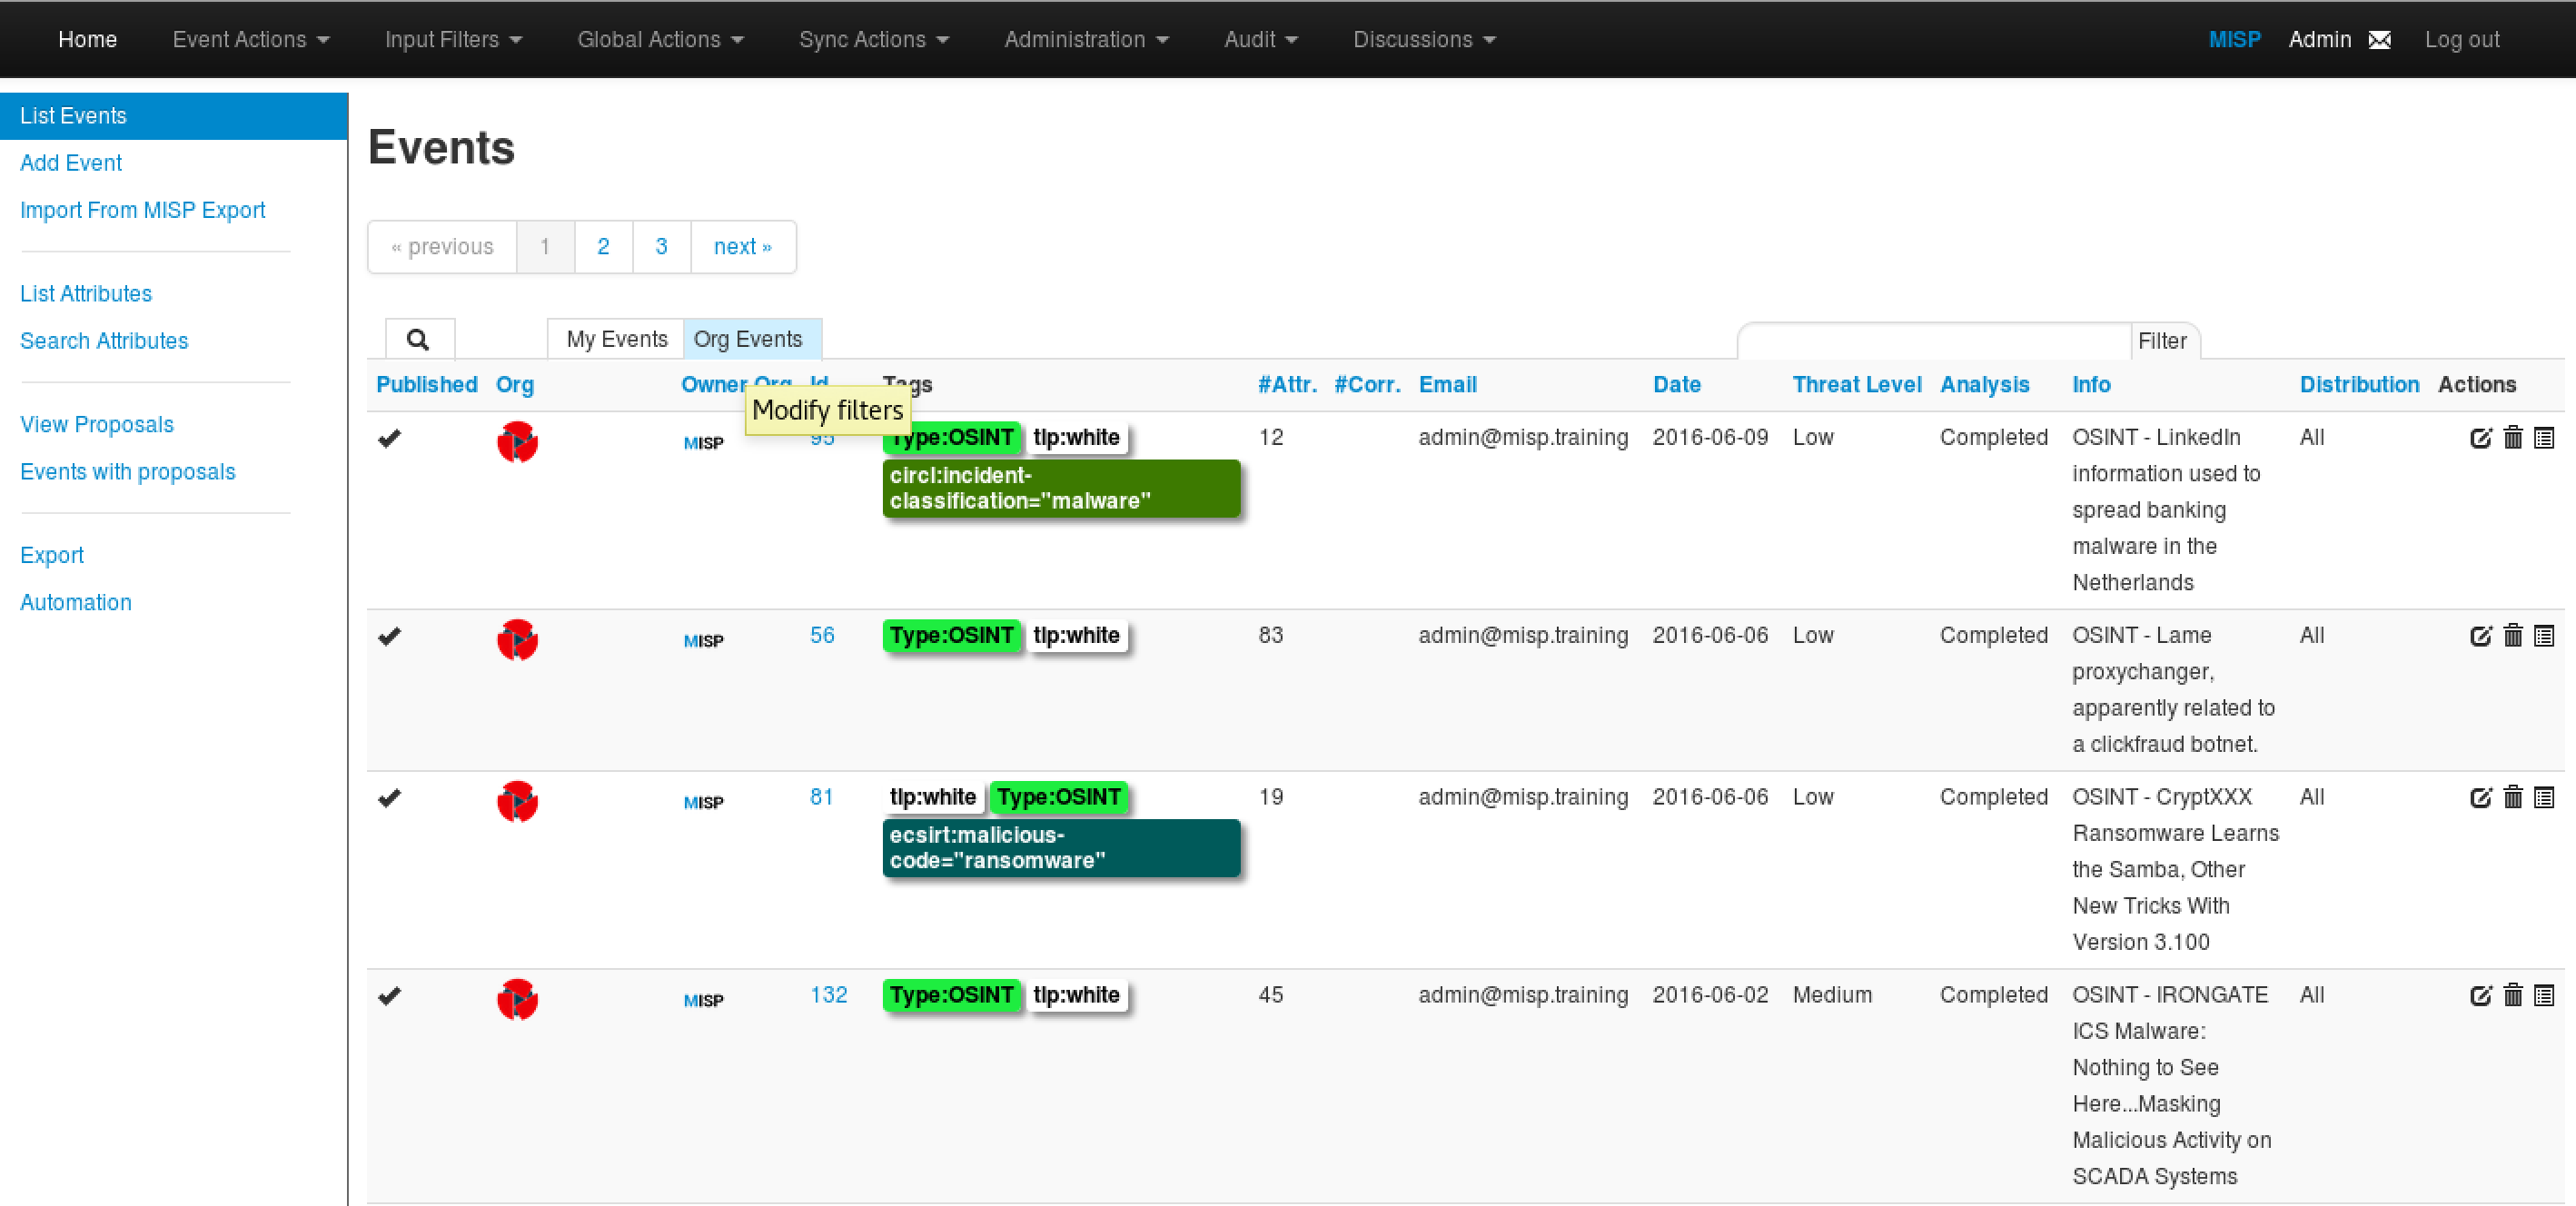
\includegraphics[scale=0.32]{res/webEvents}
		\caption{MISP : List of events}
		\label{webevents}
	\end{center}
\end{figure}


Then, by clicking on an event, we can get information on it \ref{webevent}:


\begin{figure}[!h]
	\begin{center}
		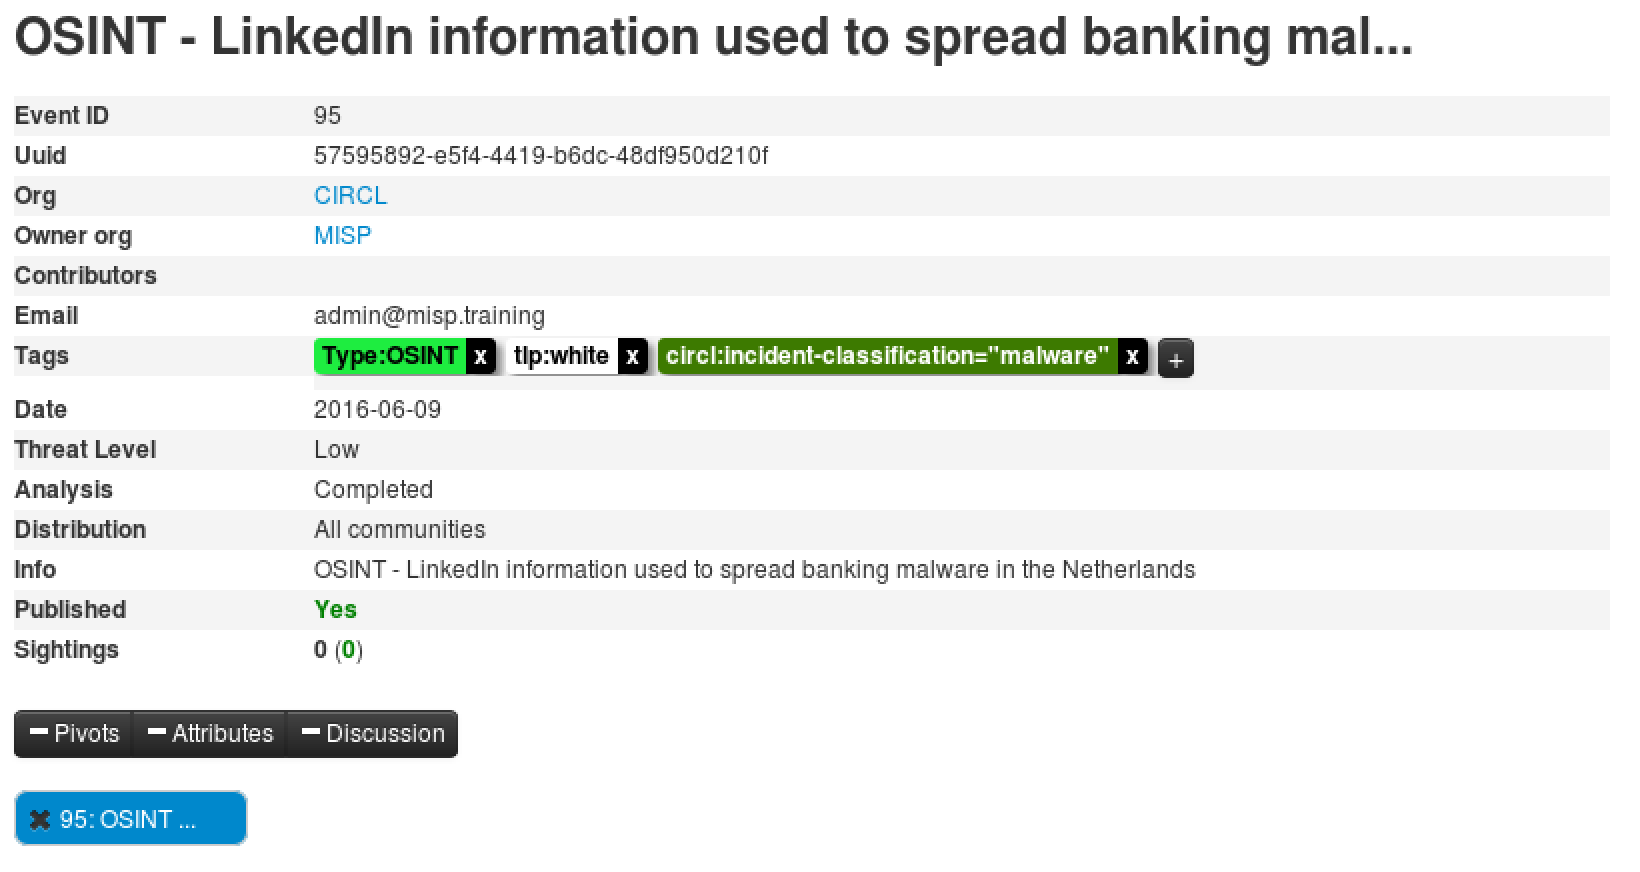
\includegraphics[scale=0.35]{res/webEvent}
		\caption{MISP : Specific information on the event}
		\label{webevent}
	\end{center}
\end{figure}


As well as the attribute list \ref{webattributes}:
\begin{figure}[!h]
	\begin{center}
		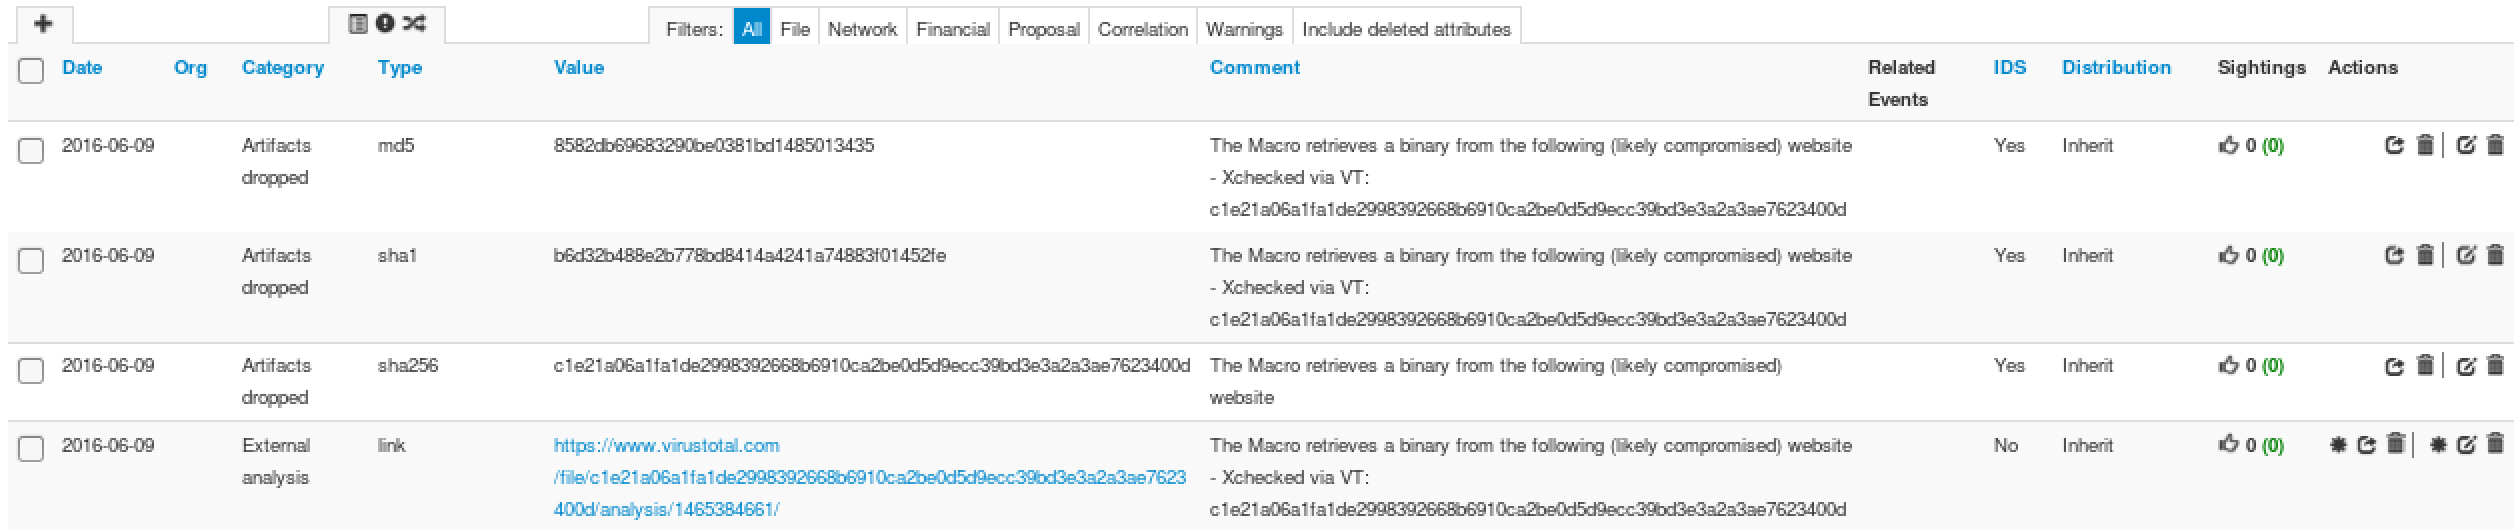
\includegraphics[scale=0.35]{res/webAttributes}
		\caption{MISP : Attributes of the event}
		\label{webattributes}
	\end{center}
\end{figure}

And the last thing that I want to show is one of the way of showing the correlations with other events and is called the correlation graph \ref{webcorrelation}:
\begin{figure}[!h]
	\begin{center}
		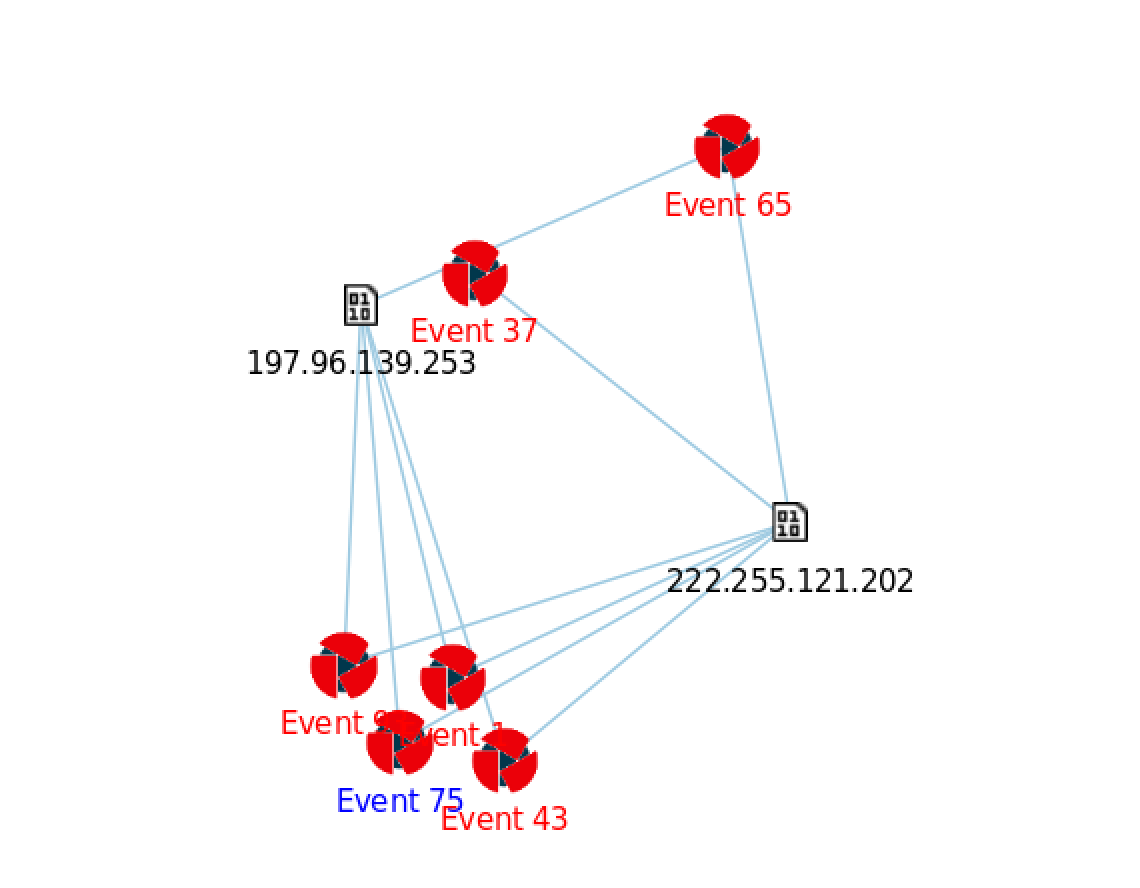
\includegraphics[scale=0.35]{res/webCorrelationGraph}
		\caption{MISP : Correlation graph for an event}
		\label{webcorrelation}
	\end{center}
\end{figure}



\chapter{Information Sharing State of the Art}

This chapter is aimed to give an overview of information sharing mostly by explaining previous works in mainly two specific domains, the first one will be about information sharing itself as well as techniques used for privacy concerns.\\
I will also take advantage of this chapter to explain the followed standards before sum up on all that this state of the art brings.

\section{Information Sharing}
As usual, a good starting point is the already made state of the art on the subject, one really interesting is done by Gregory White and Keith Harison in \cite{white2017state} where they explain the evolution of the information sharing by comparing it with the evolutions of the USA laws and their impacts.\\
Even if the analysis is about the USA, it is interesting to have an understanding of where it comes from like that the first try of sharing standardization was done just after the worm released by Robert Morris in 1988.\\
We can understand that it seems logic as we usually implement new things only when we know that it could help and here, it was the first time that they realized information sharing could have been a better and faster way to protect critical infrastructures. They also explain, in correlation with the two principal laws called the Presidential Decision Directive-63 in 1998 and the Executive Order 13636 in February 2013; how organization like Information Sharing and Analysis Organizations (ISAOs) where created with their four foundational objectives. I've sum up them as they are still really relevant:
\begin{itemize}
\item[$\bullet$] Each organization should be able to participate.
\item[$\bullet$] Development should be kept public.
\item[$\bullet$] Voluntary is not a requirements 
\item[$\bullet$] Take into account the need for confidentiality and privacy.
\end{itemize}
They also introduce the first sharing program developed by the Department of Homeland Security (DHS) which is the Cyber Information Sharing and Collaboration Program (CISCP).\\
With that, they introduce some standards like TAXII, STIX and CybOX on which I will spend more time later in their respective sections. After that, they also explain the main challenges that are facing the ISAOs. For example, the major one is a privacy and confidentially concern, any information that an organization agrees to share with others, no matter who those others are need to be kept private and confidential and only released to individuals or organizations that have a right to have access based on the agreement that are signed by members of an ISAO. This concern is really interesting as this master thesis is really on trying to ensure that property without the need of trust. What is also interesting is that they explained that privacy means that personal information about individuals within a member organization should remain private (in the context of information sharing).
While, confidentiality refers to information about organization that could lead to give others a competitive advantage.
In this article they were focus a lot on trust on trust which is one of the most important property to ensure when dealing with a sharing group.\\
We cannot share confidential information if we do not trust the other party to keep it confidential! This is already a clue on what I explained in the introduction, I want to share the information but not to give it as I'm not sure that I can trust the opposite party.\\

After that, a recent survey trying to compare the different vendors for threat information sharing was published in 2017 \cite{sauerwein2017threat}. The authors have conducted a systematic study of 22 threat intelligence sharing platforms and this article is a short sum up of their key findings I believe not always true and with a lack of example to support their say. Thus it was a general still really interesting survey even if a detailed analyze of the 22 different tools would be really welcome.\\
On the other hand, their analyze of the different types, focuses, standards and licenses used by the different platforms bring a lot of information on what should be used in todays sharing platform.\\

I've just introduce the name of some standards. They are really important as we cannot share if we cannot speak the same language. Thus these standards make possible threat sharing but also allow to make it automated. Beside that, when we decide to start in this subject. It is really too important to avoid making mistakes that perhaps have already been made. That is why some organizations like the National Institute of Standards and Technology (NIST) and the European Union Agency for Network and Information Security (ENISA) took care of publishing guidelines to help organization to involve themselves in threat sharing.\\
In Europe, the Commission recognized that they have a role to play in making the information more secure. In order to do that, they wanted to create the first pan European Information Sharing and Alerting System (EISAS on which we can find a report on the implementation \cite{eisasRapport}). For that, they have asked to ENISA to define the requirements. After that, member states that weren't yet using information sharing were really interested by and asked ENISA to develop a good practise guide based on the observation of existing exchange. This gave an intersting guide \cite{enisaguide2009} that is aimed to assist member states but also relevant stakeholders (organizations that are using communication network and information systems) in setting up and running network security information exchange.\\
In this guide, they go through setting up information sharing but they first look at the advantages and also identify laws that could get in the way. This is really important as organizations need to ensure not being recognized as a cartel or as a commercial advantage. They also focus on the trust that needs, for them, to be created thanks to regular face-to-face meetings. They also need to use TLP in these meetings.\\
Then, in 2016, NIST also published its guide \cite{johnson2014guide} that seems to me more complete and more mature. This publication is also more focused on organization than on States (unlike ENISA) and provides guidelines to improve cybersecurity operations and risk management activities through safe and effective information sharing practices.\\
For them, cyber threat information consist of IOCs, TTP (tactic, techniques and procedures), suggested actions to dectect, contain or prevent attacks and finally the findings from the analyses of incidents. \\
They go through different topics that are benefits and challenges encountered. How to establish and participate to sharing relations. Onces again, they draw attention on the importance of trust and to be compliant with legal and organizational requirements among other challenges.\\

On an other side, the paper written in February 2017 by Aziz Mohaisen et al. \cite{mohaisen2017rethinking} focus themselves on rethinking threat intelligence and to assess the risks. They argue by \cite{MalikThreat} that intelligence sharing is the only way to combat our growing skills gap in term of security. But they mostly claim that there are a lot of issues that needs to be explored in order to realize efficient and effective information sharing paradigms for actionable intelligence. They even go further by saying that understanding the risk of sharing but also not sharing is absolutely needed.\\
Briefly, not sharing is a risk as we don't receive information that could avoid us to be compromise as we can see that more and more security breaches use the same attack vectors. But in the other way, sharing information without proper restrictions may leak a significant amount of information about participant and their operation context and that can be used by an attacker to learn their vulnerabilities.\\
One solution to that is to have a very limited sharing community only with highly trusted participants. But is it really what we need to do ? If the participant are not enough, we could not get the needed information ...\\
But, if we have less trusted participant, we also need to understand to risk of leakage that could lead to both monetary and reputation loss. Taking all that into account, they propose new way of thinking for threat intelligence by defining models, communities and adversaries with their threat model.
They propose then architectural solutions as a way of assessing the quality of sharing.

\section{Existing Techniques}
Then, It is interesting to see existing techniques used in information sharing to ensure privacy and confidentiality in case where we do not want to rely on trust. This following paragraphs are then used to discover what is use and what was used before in order to get ideas on what could be implemented.\\

These articles can be divided into some sections, the first one is data sanitization, this is quite interesting even if it could not be applied in our case (as explained in a later section).\\
Then there are articles on confidential database and S2P computations.\\

One of the first article that presents some concerns about privacy in sharing security alert is \cite{lincoln2004privacy}.
More precisely, they were concerned about protecting site-private topology, proprietary content, client relationship and site defensive capabilities or vulnerabilities.\\
This was done in two steps, the first one, data sanitization, consist in removing confidential data and remove useless information. We don't take the chance of revealing information to an attacker if this one is not needed.\\
The second one is the correlation/aggregation work were alerts are linked together for analyses purpose.\\
Before explaining deeper how they sanitize data, it's interesting to first focus on how they get them.\\
 They have used three different categories:
\begin{itemize}
\item Firewalls : They consider all "deny" as a possible attack
\item IDS : They remember logs of attacks that the IDS has found
\item Anti-viruses softwares : gives also some interesting logs
\end{itemize}
They based their analyses on data coming from DShield and Symantec's DeepSight.\\

Let's come back on data sanitization, as already explained, we first remove all useless information, then, we can hash all confidential data.\\
The advantage of leaving this work to the company is to avoid the need of trust on the repository.\\
This technique is quite well working if, the data has a certain size. But, on the other hand, it is not useful for IP addresses, if an attacker is targeting a company, it has to precompute only 256 or perhaps 65536 IP address hashes. Thus this is not brute force resistant.\\
For each alert, we have two different IPs, the source IP (ip\_src) and the destination IP (ip\_dest). We can classify all these IPs in two categories:
\begin{itemize}
	\item Internal IPs : IPs that belong to the company
	\item External IPs : IPs external to the company
\end{itemize}

The first category is, of course, the one that we want to protect and in order to do so, these IPs are hashed with a keyed hash function like HMAC. While the second type is hashed by a simple hash algorithm like SHA-1.\\
The result is that we can compare all SHA-1 hashed IPs together while only companies can decrypt their own internal IP addresses.\\
It is an efficient technique as they receive millions of IPs at all the time. And, as the attacker is not able to see if the IP is hashed by HMAC or SHA-1, he has to test all hashed IPs against a precomputed table which is not feasible.\\
They are also using another set of protections like the randomized threshold for publication of an alert but it goes out of the scope of this work.\\
In sanitization, the also round all timestamp to the nearest minute in order to add some uncertainty!\\
The second step is the correlation, they spoke about historical trend analyses, source/target-based analyses and event-driven analyses but some other articles are more interesting for the correlation principle, thus I'm not going deeper in it.\\

Then, \cite{xu2005privacy} was also working on confidential data sharing starting from the first article, but they came up with a new interesting idea, instead of hashing confidential data, why not generalize it and do probabilistic correlations.\\
(They also used a technique to create probabilistic attack scenario which is a set of alerts that are put together to create a bigger attack).\\
\textbf{Guided alert sanitization with concept hierarchies:}\\
For example, if we have an IP 192.168.1.123/32, we can generalize it to 192.168.0.0/16.\\
The depth of the generalization is chosen thanks to the entropy or the differential entropy technique explained in \cite{cover1991elements}.
\\
\textbf{Alert Correlation:}\\
They focused on defining similarity functions between sanitized attributes and building attack scenarios from sanitized attributes
\\

This article was interesting for seeing a technique of data obfuscation. And then to create correlation analyze but, it's difficult to apply that technique in order to create a database of still usable data for prevention or detection !
\\

I've explained some solutions that can be applied to IP addresses or file (just hashing them). But, what if we could do the same with all network packets and still getting some privacy!\\
That's the goal of \cite{parekh2006privacy} ! Today, it's not enough to analyze IPs, URLs and so on. We need to go deeper in it, that's why they propose a technique based on the byte distribution of the packets.\\
They used PAYL and Anagram \cite{wang2006network}, systems that they have created and which are really useful in these analyses.\improvement{To remove ??? => Check articles}\\

Sanitization is used to protect information by keeping privacy, but, as \cite{mohaisen2017rethinking} is referencing, there are other ways for sanitizing data. Some of them are k-anonymity \cite{sweeney2002k}, l-diversity \cite{machanavajjhala2007diversity} and the key privacy guarantee that has emerged is the differential privacy \cite{dwork2008differential}.\\
First, k-anonymity is an attempt to solve the problem of anonymizing a person-specific field structured data with formal guaranteed while still producing useful data. A dataset is said to have the k-anonymity property if the information for each person in the dataset cannot be distinguished from at least k-1 individuals. This is done by removing attributes or by generalization as seen earlier. But this technique was unfortunatly performing poorly for certain applications. Thus, l-diversity was an extension to it in order to handle some of the weakness of k-anonymity. It does that by increasing group diversity for sensitive attributes in the anonymization mechanism.\improvement{Read cited articles instead of simple the first article to be sure of my understanding}


As confidentiality and privacy are such a big deal, could we only share data when there is mutual benefits ? Yes and it is what will be done in the master thesis but there are also existing techniques where each organization are able to do some secure two-party computations with others.\\
The interest is to get some metrics, for example, if there are only IPs in the databases, if we can get the intersection or even only the cardinality of this intersection. That is, if it is non-negligible, we know it could be interesting to share with them!\\
The paper written by Freudiger et al.\cite{freudiger2015controlled} focused on this problem by working on a DShield dataset. They've experimented some strategies to know if it could be useful to share or not with another organization. And then, they also experimented to share the whole dataset of the company, only the data set linked to the intersection just found or only, the intersection (just to get a rough idea of what they have in common ... ).\\
Their conclusion were intuitively expected but still interesting :
\begin{itemize}
\item More information we get on an attacker, the better the prediction are.
\item The chosen collaboration strategy has a really big impact (some of the strategies are really useless).
\item Collaboration with companies improves not only the predictions but also removes a lot of false positive.
\item Sharing only about common attackers is almost as useful as sharing everything.
\end{itemize}

\info{Mutiparty private matching peut aussi être interessant dans mon domaine non ?}

Now that we see more concretely what is information sharing, a good question is to understand it is used in todays system. A usual way of using the information is via Intrusion Detection System (IDS). Contrarily at what we could think, IDS are as important as Intrusion Prevention System (IPS) as all analyses cannot be done in real time and moreover, new information on new threats could appear latter on thanks to sharing or other ways. This could then allow to discover the attacker, even if he is already in, we need to discover him as soon as possible! Analyses had shown that the mean time an attacker stay in the system before beeing detected is about 200 days which is unbelievable.\improvement{Find article about it}
\info{Parler un peu des IDS .. }



\section{Standards}
As we want organizations to share threat informations, we need them to "speak the same language" or more formally, to use the same standards.\\
For that, we can categorize the standards into four categories (lists of other existing standards can be found in \cite{AwesomeTreat, mohaisen2017rethinking}):
\begin{enumerate}
\item Enumerations
\item Scoring Systems
\item Languages (CybOX, STIX)
\item Transport (TAXII)
\end{enumerate}

I will only focus on the three that I've cited before as we can see in \cite{fransen2015cyber, sauerwein2017threat} that the most promising standards for a threat sharing intelligence sharing infrastructure are CybOX, STIX and TAXII. They have been developed under coordination of the MITRE Corporation and have very strong momentum in adoption by industry leaders and threat intelligence communities such as the Financial Services - Information Sharing and Analysis Center (FS-ISAC).\\
The  Structured Threat Information eXpression (STIX) \cite{barnum2012standardizing} provides a language to represent cyber threat information in a structured manner and is really interesting as it provides a structure to express a wide set of contextual information regarding threats in addition of the IOCs. The complete list is :

\begin{itemize}
\item[$\bullet$] Cyber Observables
\item[$\bullet$] Indicators
\item[$\bullet$] Incidents
\item[$\bullet$] Adversary Tactics, Techniques, and Procedures (including attack patterns, malware, exploits, kill
chains, tools, infrastructure, victim targeting, etc.)
\item[$\bullet$] Exploit Targets (e.g., vulnerabilities, weaknesses or configurations)
\item[$\bullet$] Courses of Action (e.g., incident response or vulnerability/weakness remedies or mitigations)
\item[$\bullet$] Cyber Attack Campaigns
\item[$\bullet$] Cyber Threat Actors
\end{itemize}

 Moreover it tries to stay as "human-readable as possible". And the chapter 9 of \cite{barnum2012standardizing} may be really interesting to spend time on it. It explain in detail the structure of STIX.\\
 For expressing the observable, STIX is using Cyber Observable eXpression (CybOX)\cite{barnum2012cybox} that allows to state the specification of events or stateful properties.
Then, we need a transport standard which is the Trusted Automated eXchange of Indicator of Information (TAXII) \cite{connolly2014trusted} .


\section{Sum up}
When I started the master thesis, my knowledge about threat information sharing was clearly none. I had to look up for articles and information where I was able to find some. I've finally chosen some articles and some points that I found interesting to share in order to understand the different step I followed and the different ideas on which I thought about.\\
Also, I've spoken about MISP as it is the platform I'm interesting on. There is an available really good awesome list \cite{AwesomeTreat} available where all different existing standards, tools and techniques available in this domain.\\
But in order to come back to MISP. The main advantages compared to the proprietary solutions (like Soltra Edge) is that :
\begin{itemize}
\item[$\bullet$] Transparency in term of code and of the contributor.
\item[$\bullet$] Quantity and diversity of connected entities
\item[$\bullet$] The price and the non-existence of entrance barriers
\end{itemize}
On the other hands, there exist also other kind of sharing types like DShield but they are sharing the whole bench of indicators and deals with a lot of data while MISP is more interested in events and in the analyses of what is going on.\\

The difference between privacy and confidentiality had been well explained but I want to add that here, when I speak about anonymity in sharing, I mean that what would be interesting would be to have a way of sharing what is going on without the need of sharing who had seen the indicators.//
Then, I could find a lot of techniques in order to generate blacklists, detect event correlations and protect companies with it.\\
In the state of the art, I've also spoken about attack scenarios and cardinality of intersection to evaluate the benefit of sharing before doing it. These kind of techniques are not yet implemented in MISP but could appear one day.\\

As discussed with the risk, there are a lot of privacy concerns about sharing data. And thus, a lot of separate techniques. But there is an additional important problem that we need to take care of. For example, one of the solution for preserving privacy was simply hash the data. For big sized data, It's not feasible to brute force in order to get back the information but, for IP addresses, since in general, there are only 256 or 65536 IP addresses for a specific company, we could create a table with all possible hashes and test them all!\\

Then, it was really useful to see these existing techniques but it unfortunately does not mean that it could solve all of our problems. They had other purpose when designing their solutions and it can lead to some disadvantage in what we are attempting to do.\\
For example, Bloom Filters are a really good idea but they are not enough by their own has they do not give data at the end but just a probability of a specific IOC to belong to a specific set.\\
On the other hand, sanitization is not good for us either as we would lose all the interesting data with the explained techniques. Noise is thus not a valid choice either.


\section{Where did it lead me ?}

We have a data set of malicious data, IOCs, events and we want to share them. This is what is already done by the MISP project. But now, what if we want to distribute these information by giving the data set to an organization without having to trust her?\\
It would be really nice, computer specialists would be able to check on computers to discover infections, problems and moreover learn how to fix it thanks to the previous analyses contained in MISP. But there is still a problem, some information are confidential and we need to have some privacy concerns while sharing. \\
Actually, if a company discover information on its system, why should they share it ? They already have been compromised and sharing could give useful information to an attacker, as the company topology ... \\
But if they do not share, why other should accept to share with them ? That is why, actually all sharing groups rely on trust. Here, the trust must be replaced by something else.\\
Sanitization is a good idea but, it would modify data up to make them unusable for every one.\\
What then if we could find a way to share only if the user has really knowledge of the event and can share information on it as well, or is really infected by and need help that could be given by the information.\\
I will consider this problem but with two different kind of solution. The first part is when the database could be shared because an attacker could not get information from it (Easier to get data, so perhaps we cannot put all data on it).\\
And the second approach is one that still need a server to respond but allowing more privacy.\\

But still, the idea that a common user have access to data while an attacker, which is a specialist, cannot seems infeasible in a lot of cases. The attacker always ends with the data but, if he takes 1 second, 1 day, 1 week, 3 months or years is different because, we can then think about how long a data is valid? \\



\section{Misp-Worbench - hashstore}

Misp workbench\footnote{https://github.com/MISP/misp-workbench} is a set of tools to export data out of the MISP MySQL database and use and abuse them outside of this platform.\\

They have already implemented a privacy aware tool called hashstore. This was implemented in redis\footnote{http://redis.io}. This is working by creating a dataset of all hashed IOCs. And then by the use of the redis server, we can use a redis client to request data.\\
Like that, if you want an information on a particular IOC, you need to already know it to be able to take its value's fingerprint and make the request.\\
On the other hand, coming back on the small data problem, if we consider an attacker that want to try every possible IPs, for IPv4 it represents 4.228.250.625 different IPs that needs to be tested. Even if it is a lot it is still feasible as redis is really fast (The attacker even pipeline its requests\improvement{Check that, I think that it was not feasible in the system but I need to check why})! Moreover, not all IPv4 need to be tested, for an example we can avoid private subnet like 10.0.0.0/8, 172.16.0.0/12, 192.168.0.0/16 which already represent 17.891.328 addresses.


\section{Limitation}

What we want ? A way to share information only with people that has already some information or that are facing the related event. It would be amazing to do so but it would mean to make available a dataset where we could allow them to query.\\
The hashstore was a great idea as we need to now what we are looking for to request but, for a small data that could have only 10000 possibilities. What if the opposite player try ever 10000 possibilities to get what we know? \\
We could make a limitation on the allowed number of request but, a system that would like to check everything that it sees on its network should still be allowed. Could we differentiate both ? \\
So if we want to make the task more complicated for the attacker, we need to make it more complicated as well for the authorized used. This is quite difficult because if we make it infeasible for the attacker, we are also making it infeasible for the user as, with the example, there is only a 10000 factor between legal utilization and an attack.\\

We thus know that it is intrinsically impossible to fully hide small IOCs while still allowing a subscriber to evaluate the rule. But we want to find a solution that could be an approach this problem.


\chapter{Implementation Ideas}

Now that the subject seems clearer, there are a lot of different possibilities that could be explored. This chapter will be the opportunity to dwell on some of them in order to compare their strong points as well as their weakness.

\section{Bloom filter}
Bloom filter is a space efficient probabilistic data structure  used to efficiently test the membership of specific values.\\
If a dataset is only used for testing the membership, instead of storing the whole dataset that could be really large, we can use a bloom filter structure that use less than 10 bits of memory per element with a 1\% rate of false positive which makes it space efficient.\\
A simple example to show the interest could be a data set of all the students' name and surname at university. Taking the hypothesis that each name and surname has approximately 6 characters and that there are about 20 000 students ( Harvard ). The dataset should use 20 000 * 6 * 2 * 8 (=1920000) bits while a 1\% false positive bloom filter could be only about 20 000 * 10 bits which is already 9 times smaller for such a small data example.\\

\subsection{Data Structure}
A bloom filter is a m bits array (fig. \ref{bloom-1}) all set to 0 at the starting point. Beside that, there are also k independent hash functions. 

\begin{figure}[h!]
	\begin{center}
		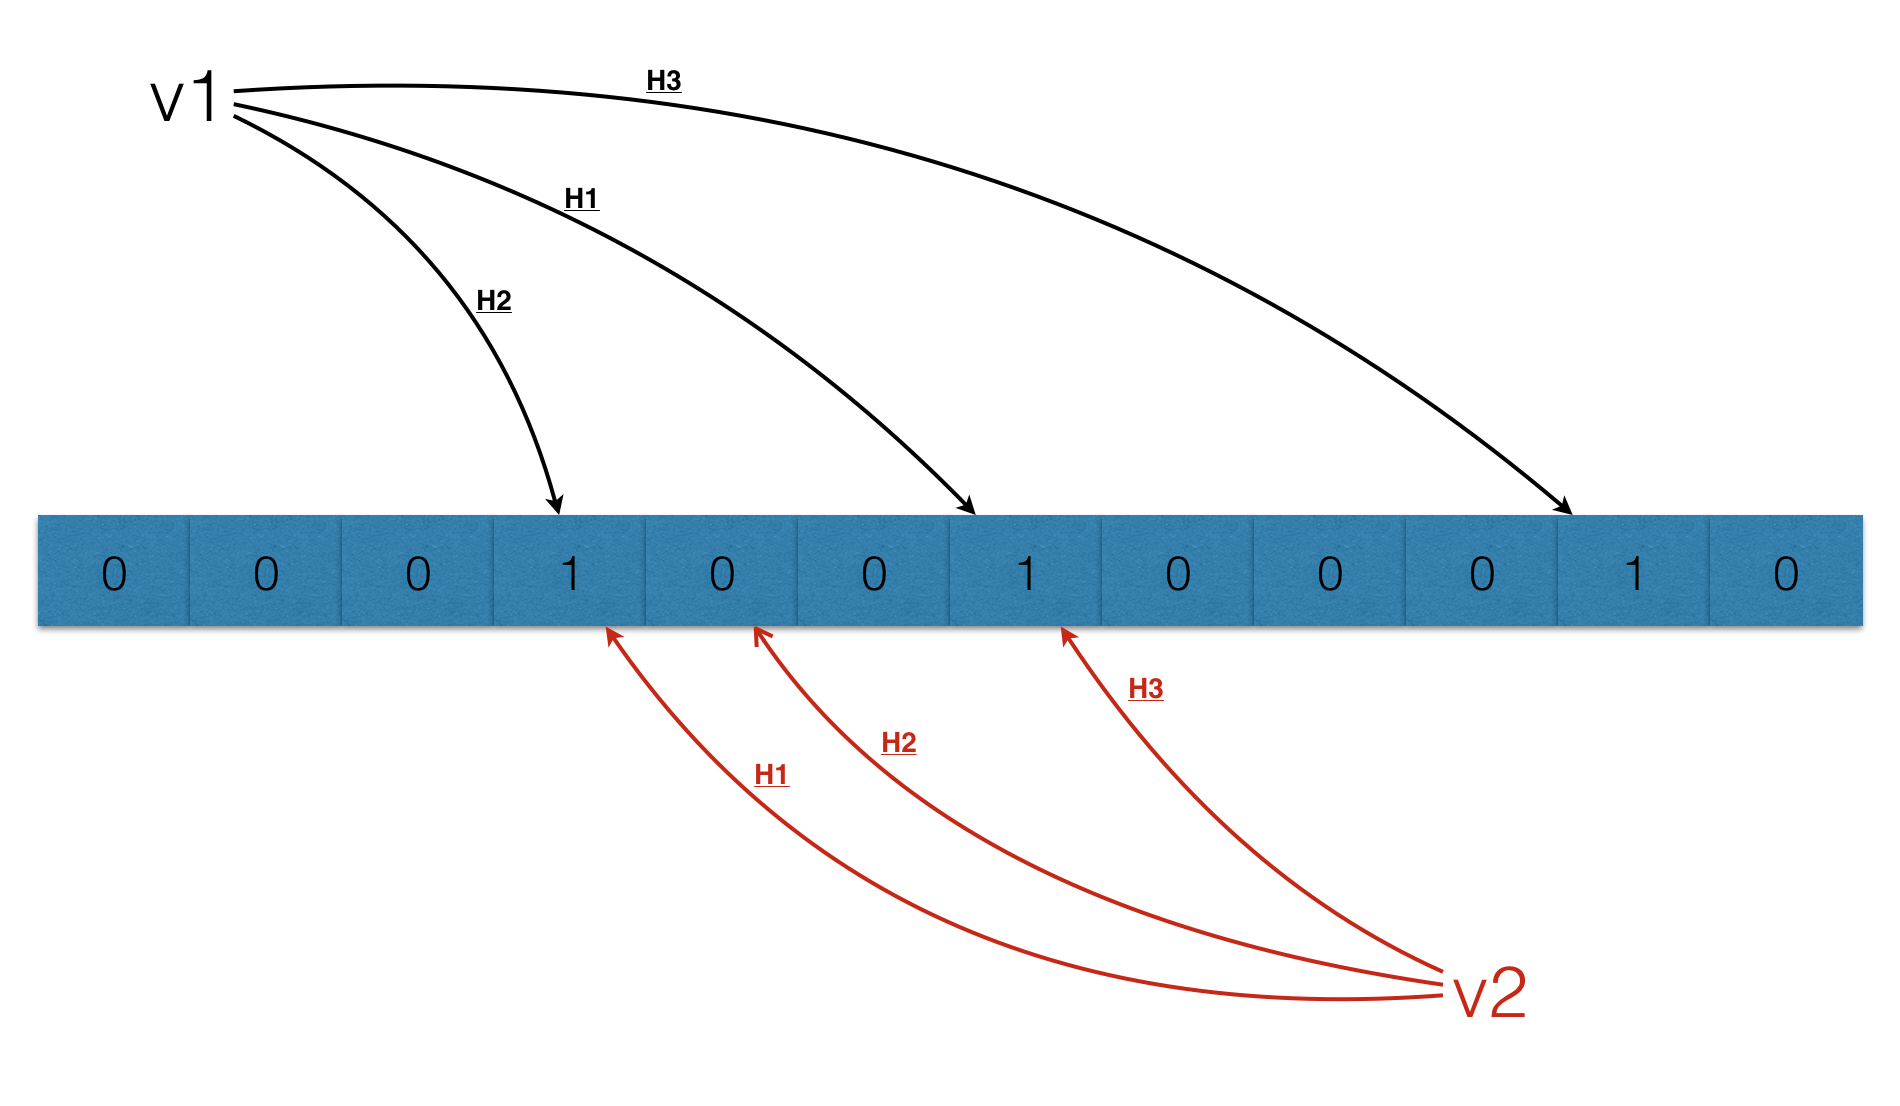
\includegraphics[scale=0.3]{res/bloom-1}
		\caption{Structure of a bloom filter with m=12 and k=3}
		\label{bloom-1}
	\end{center}
\end{figure}

To add the value v1, each hash function gives an index where we set the indexed bit to 0. In the opposite, if we want to test a value for membership, we have to check all indexes given by the hash functions. As we can see on figure \ref{bloom-1}, v2 is not in the set.

\subsection{False Positive}

Bloom filter is a probabilistic data structure as when we are checking for a value, either the value is \textbf{not} in the set or is \textbf{perhaps} in the set. \\
In the latest case, this is due to false positive where all the k hash functions gives indexes already set to 1 (fig. \ref{bloom-2})while the element should not be in the set.\\
Even if this could be annoying that is what could make that data structure interesting while trying to to reveal the whole data set.
\begin{figure}[h!]
	\begin{center}
		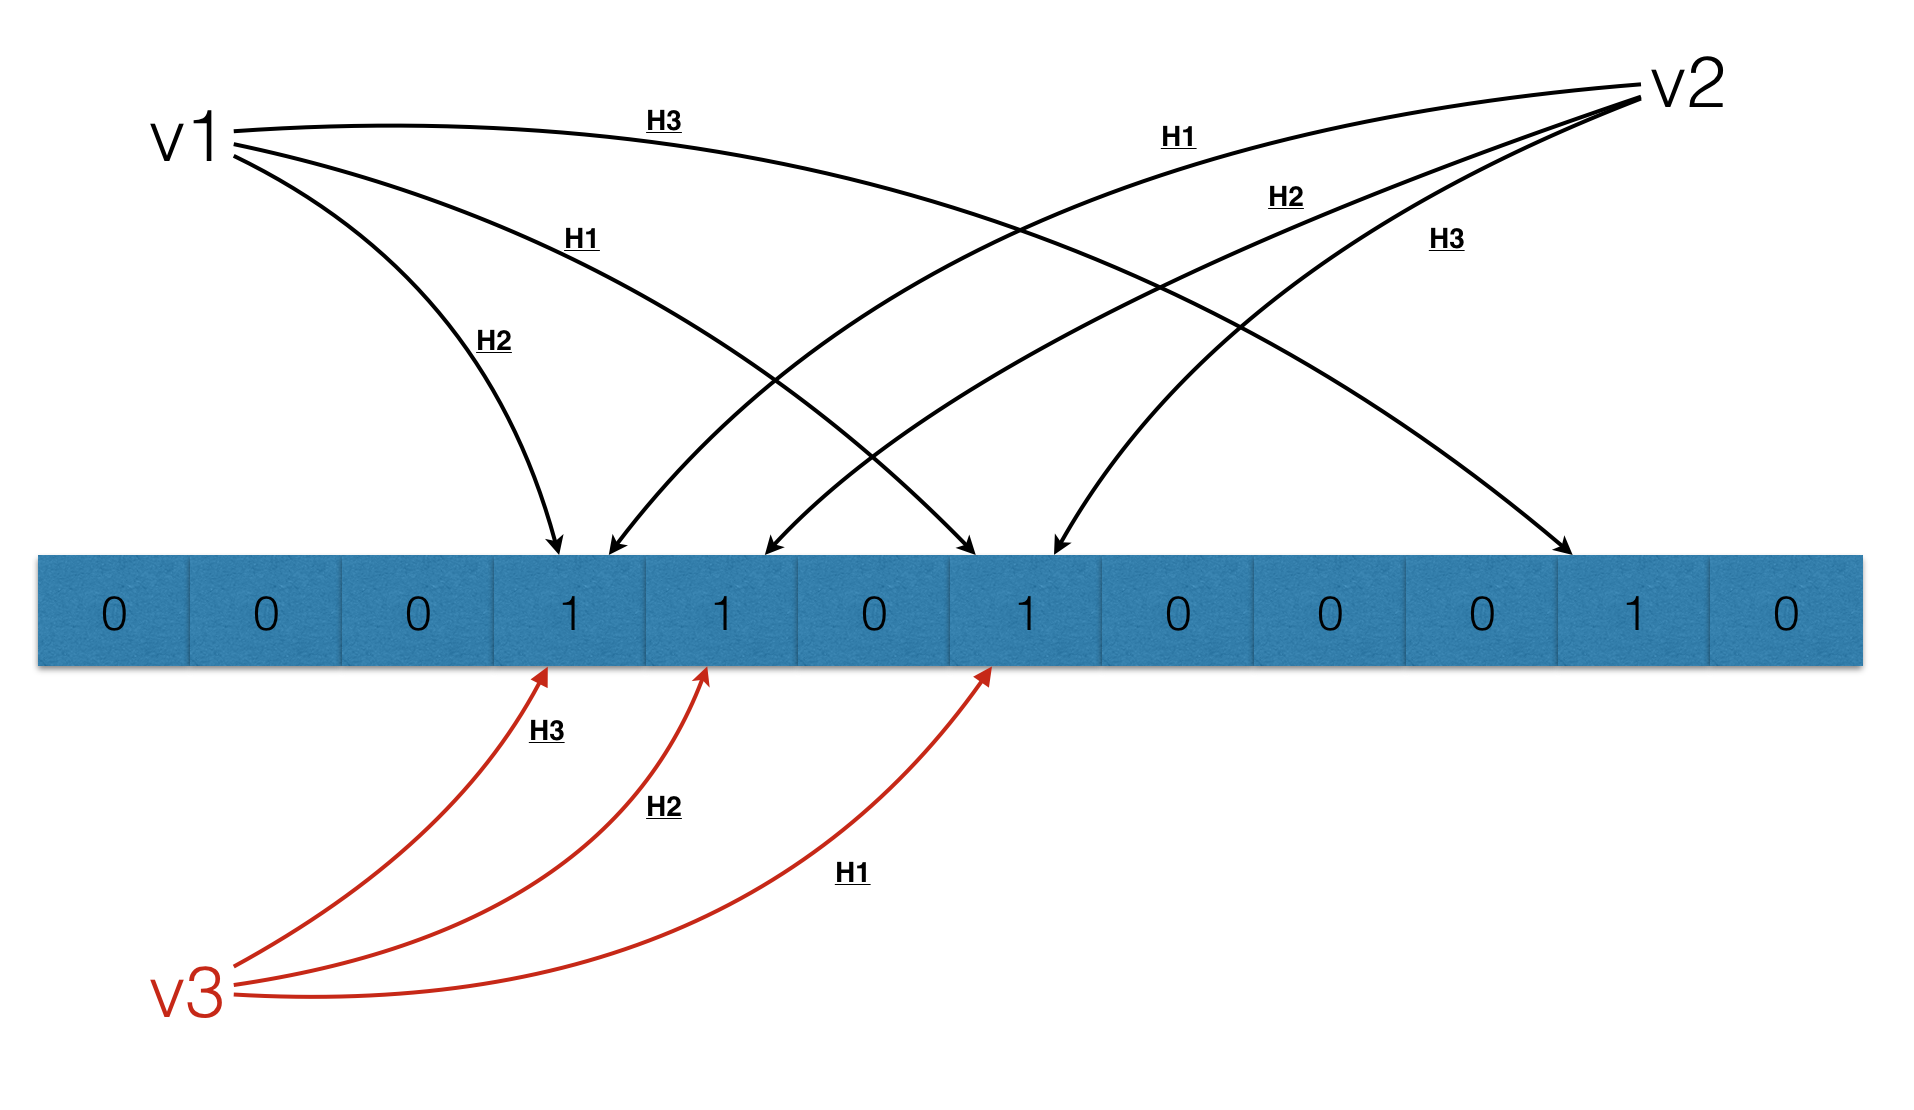
\includegraphics[scale=0.3]{res/bloom-2}
		\caption{False positive v3 in a bloom filter with m=12 and k=3}
		\label{bloom-2}
	\end{center}
\end{figure}

\subsection{Control False Positive Rate}
If we check for a value in a bloom filter, at the end, we only know if it is not in the set or a probability to be in the set. Playing with this probability could be interesting for hiding some informations. \\
If the probability is about 50\% in ip, it loose all interest for an attacker to brute force attack as at the end it would give him no information. While, for a real user, requesting for one ip could still bring some information for example knowing that an element had never been signaled before.\\
This is why it could be useful to get more information on the false positive rate and how we could use it.\\

If n is the number of element inside the data structure we can approximate\footnote{https://en.wikipedia.org/wiki/Bloom\_filter} the false positive rate by $(1-e^{\frac{-kn}{m}})^k$ but a more useful is to define k in function of the willing rate for the false positive. In this case, we can notice that k is independent of the number of element inside the set while on the opposite, it is m who need to change in function of the number of values n:
$$m = - \frac{m\ \ln(p)}{\ln(2)^2}$$
$$k = - \frac{\ln(p)}{\ln(2)}$$
(These are approximations)

\subsection{Bloom Filter could Leak Informations}
It could seems useless but nevertheless it could have huge impacts. If we create bloom filter and we ensure a false positive rate, with the size of the array (m) and the number of hash functions (k). An attacker could approximate the number of values in a bloom filter like shown by Swamidass et al. \cite{swamidass2007mathematical}:
$$n* = - \frac{m}{k} \ln\left[1 - \frac{X}{m}\right] $$
with X the number of bit set to 1.

\subsection{Could it be useful alone ?}
It is not enough alone as we not only need to test element for membership but we also need to get back information if it is. Moreover, when developing a system with bloom filter we need to take into account all small data that could leak. \\
But it is still an interesting solution and twinned with the later explained implementation could have great benefits.

\section{Machine Learning}

Machine learning is \textbf{the} actual technology for security. A system that could evolve and learn by itself. No need for updates! \\
And as the conference "Beyond the blacklists: Detecting malicious URL through machine learning" showed at the Black Hat Asia conferences, it can work.\\
They focused on URL lexical feature like the url length, vocabulary, path, hostname, parameters, http headers (in average, there are less fields with malicious connections) and they manage to get a 84\% detection rate on  about 750K malicious URLs which is really promising.\\

But on an other hand, Machine algorithm also brings false positive like in bloom filter but also false negative.\\
Even if a false negative could be really bad, it could be use to protect our data.\\
Here, we don't want to be able to discover new malwares but we want the same as with bloom filter, knowing if an element belongs to a set.\\
With this objective in mind, the goal would be to analyze the impact of false positive and false negative while training an algorithm that like a decision tree as, in this particular case, overfitting is a property that we need.\\
Then it could be interesting to check the base concept representation (BCR) to analyze if this technique could be interesting. \\



\section{Secure Multi-Party Computation}
In our case, we could imagine, an organizations with informations to check if it belongs to IOCs of other organizations.\\
Each organization possesses its IOC database and is not ready to share all their informations. But, once again, if it could help an other organization to solve its problem, they agree on sharing only these informations.\\
That is where Secure Multi-Party Computation could play a role as there are techniques to find the intersections of 2 datasets. This is also called private matching \cite{agrawal2003information, li2005private}.\\

This technique could be really interesting but has the disadvantage of heavy computations on both side.

\section{All in one request}
Here the goal is quite different, Imagine the case of a forensic detection of what had gone wrong.\\
We can do it differently, we do a full analyze of the machine, then, once we have the whole data set that we want to test, we send everything and the data system just answer with the id(s) of the triggered event but we don't know what triggered it thus we don't really know the content.\\
In order to avoid brute force, we could allow only a limited amount of request per day with a limited amount of data.

\section{Proof of Work Database}
This idea is to slow down brute force attack thanks to proof of work. Even if this idea is one step closer to the final implementation, it is still different by the need of a server to communicate with for each requests.\\

Here, we want to keep a database, we don't want any false positive nor false negative. But by doing that, we make our database available to brute force attacks.
But we can try to avoid that or to make it more time consuming by adding computation.\\

A possible implementation could be one we a random key chosen by the database server. This key could be regenerated with a small period and also every 1000 thousands requests.\\
On the other hand, the client should brute force this small key each time it has changed. This slow down brute force attack while still be useful for a user that is doing less than 1000 requests to test its system.

For example, a possible request message for an ip could be : hash(IP)||hash(IP||key)\\

The idea is interesting by is still not bullet proof against brute force attack. And also need a server to respond at each request.

\section{Conclusion}
I've explained some basic ideas that could lead to different implementations, lot of work are done especially on private multi-party matching that could lead to the best option if requests are rare or, for example if it is used to periodically compare and synchronize data related to the same events between MISP instances.\\
Nearly all solutions still needs a server that we would like to get rid of (After the data had been generated) and for that, a machine learning model or bloom filters are the right track.

\chapter{Implementation}
I've explained ideas in the previous chapter, some of these could be implemented. But a nice article \cite{van2016private} was published in the few first months of my work and they had found a technique that could also work for us as their goal was similar as they say that they propos a technique that allows parties to share information without the need to immediately reveal private information.\\
Their implementation was for bro, here I will make an implementation working with MISP and improve its matching properties and the modularity of the code. \\
By modularity, I mean that I to be able to add what I will call cryptographic modules in order to test different techniques with the same code.\\
In this chapter, I will first explain their article, then the modifications I've made with some improvements.\\
A discussion on the libraries and tools will follow before benchmarking test with discussion on the implementation.

\section{Private Sharing of IOCs and Sightings \cite{van2016private}}
This paper consider a cryptographic approach to hide the details of an indicator of compromise. They consider two different phases, the first one is sharing these IOCs while the second one is to privately reporting the sightings of IOCs.\\

The second could be really important as explained before to monitor the events and attributes in MISP.\\ 
Moreover MISP had now the possibility to add sightings but their technique seems not efficient enough and really difficult to implement in MISP. I've got some other ideas but I finally only focused myself on the sharing part as it is not yet totally clear how the feature will be synchronized between organizations and other instances.\\ 
But still, It could be an important and really useful further work to do.\\

But before starting, they warned the reader as I did in the limitation section, that using these cryptographic function is better than not using them at all but is not a miracle technique as it is theoretically impossible to hide the IOC’s content in the used context (Subscriber receive the data to check on its system).\\
Additionally, it has a performance cost but in my beliefs, it worths it.\\ Their implementation was also in the source-subscriber information sharing model which fits our model where MISP is at the center.\\
First, they define an IOC as rules that are propositional formula where the propositional variables are defined over features or observables like Internet Protocol (IP) or fingerprints of malicious program (but it could be any categories of MISP). They also claim that every rules (IOCs) can be expressed in the Disjunction Normal Form (DNF) without any negation (e.g. destIP= 198.51.100.43 $\land$ destPort = 80).\\
Hereandafter the value is considered has the concatenation of all values of the IOCs contained in a rule : IPv4$||$port\_number. It has two advantages, the first is to represent the complete rule and the second one is that it can be a little more difficult to brute force as it is longer and types can differs.\\

\begin{figure}[h!]
\begin{center}
	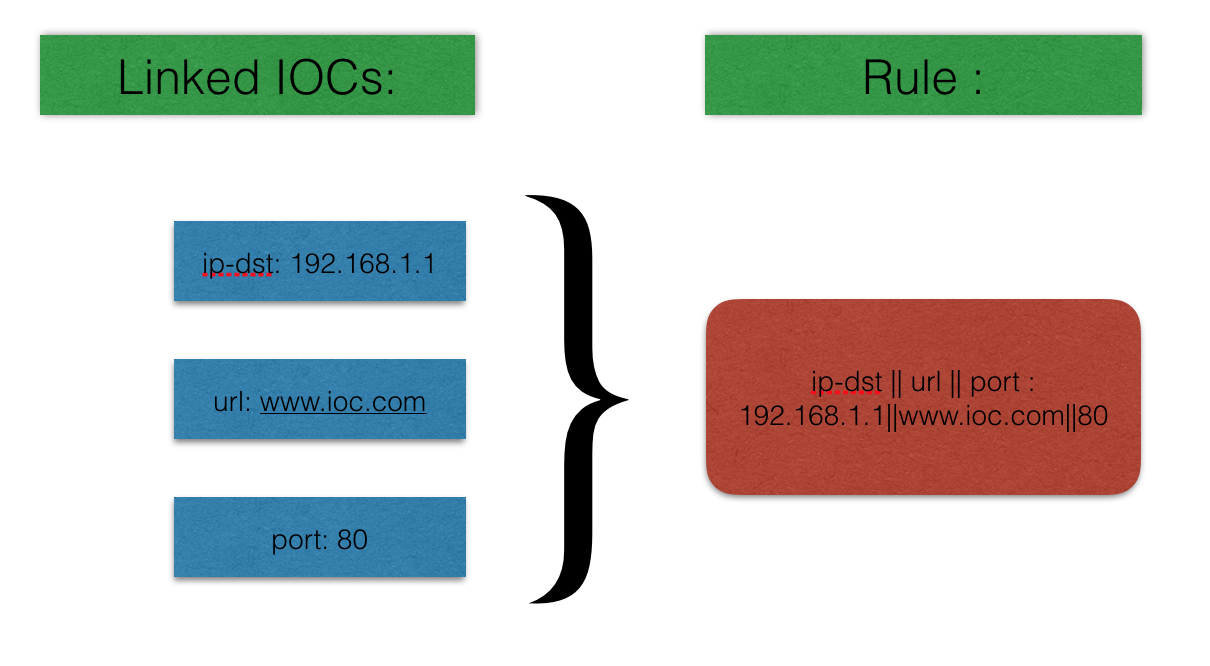
\includegraphics[scale=0.5]{res/ioc-rules}
	\caption{IOCs transformed into a rule}
	\label{IOC-To-Rule}
\end{center}
\end{figure}

So, now, we have a rule that can be checked on computers but, what is needed is the other party to be able to check it while keeping the IOC's content hidden and that is where it becomes really interesting.\\
As it has to be useful, they have obfuscated the values while keeping the structure of the rule in clear. The basic idea is thus to hash the rule's value. For a subscriber, it is still usable as he only need to hash its data to check for a match. But, in this way, we are doing the same as in the hashstore already explained and there is thus a lack of protection since every individual feature variable can only take a limited set.
Thus we could face an attacker that would succeed with a TMTO attack or a complete precomputed table.
For solving that, they are using a non secret salt value chosen at random for \textbf{each} rule (IOC). Beside that, the attacker time can be increased as well thanks to the cryptographic hash function used. The second part is really affecting the honest subscriber performance as well but is needed to slow down enough an attack.\\

But they didn't stop there, considering all these ideas, they have added the possibility to include a Course Of Action (COA) message with each rule. This is the real advantage compared to bloom filter. The output is precise, there are neither false positive nor false negative and additionally, a match can give the interesting data to the honest user.\\ To do so, instead of hashing the combined values, they use it as input for a key derivation function (KDF) that generates a key used for encrypting the message in the rule.\\
Thus this new type of rule, instead of obfuscating the data contains, the type of value (as before), the salt used for the rule and the encrypted message.\\

\begin{figure}[h!]
\begin{center}
	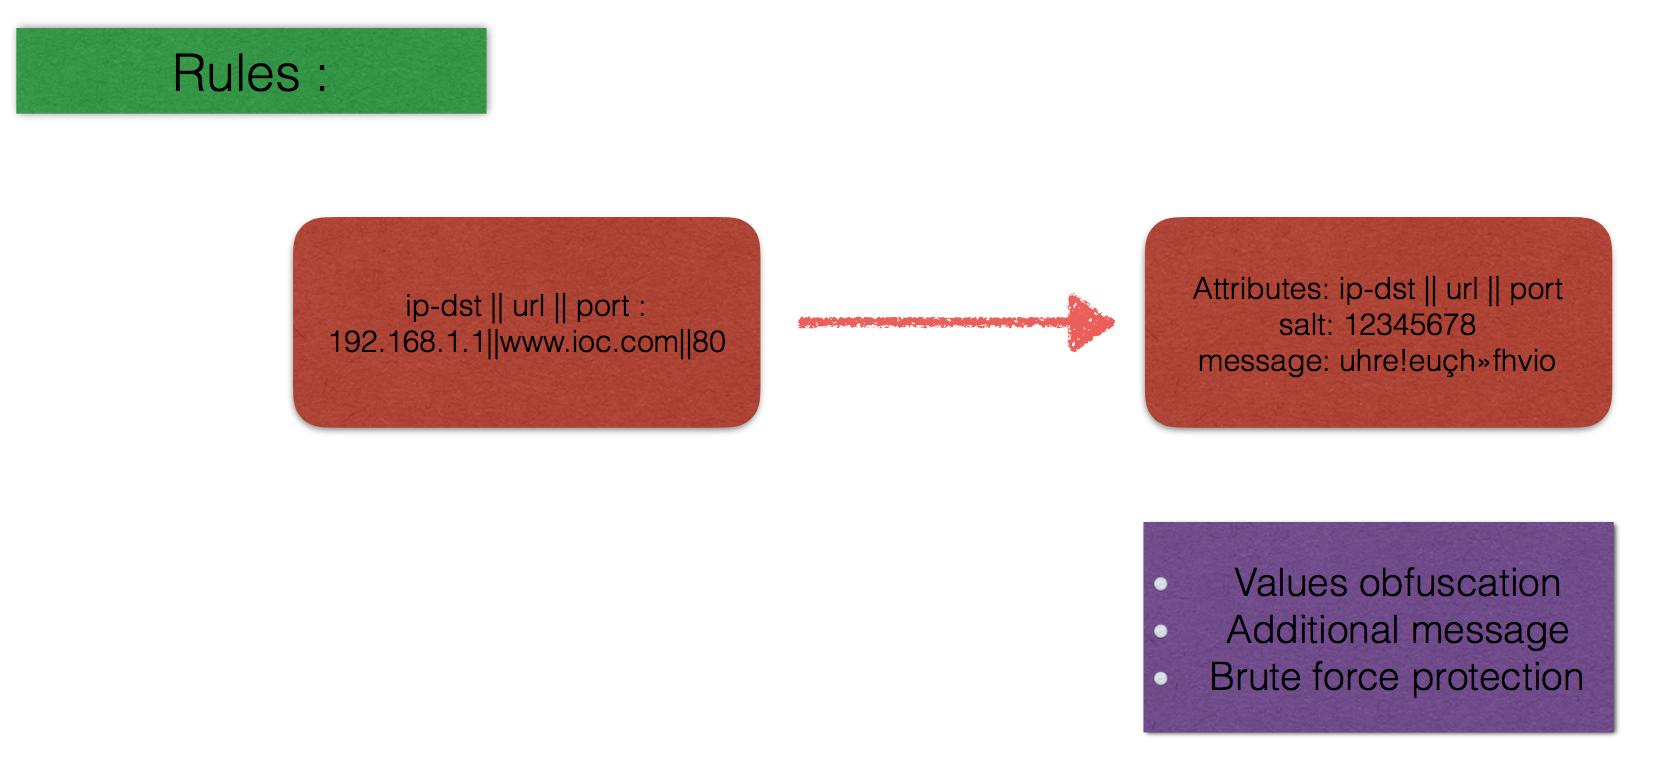
\includegraphics[scale=0.3]{res/obfuscation-rule}
	\caption{New format for the rules}
	\label{Obfuscation-Rule}
\end{center}
\end{figure}

Trust is one of the major problem in information sharing and is discussed in all standards, guides and articles. Here they have an attempt of solution that could really work. As a user cannot normally decrypt the complete rules data set, if for each generated rule, we add a source identifier used in each rule in the KDF. If a set of rules is leaked, we can now trace it back to the offending user. \\
This little additional feature may seem to be a detailed, I'm intimately convinced that it could help organization to decide sharing more confidential data as they could turn themselves 
again the leakage source in case of problems which could limit the cost damage as well as the reputation damage. Moreover, in MISP there is also an identifier that could be used and moreover that need to be kept private which is called a Token.


startPad = '\\x00'*16
\subsection{Create a rule}
\begin{itemize}
\item Create a salt and an iv
\item password = all IOC's value joined by a comma
\item create the key with from the salt and the password
\item encrypt the message (CAO) in (aes, ctr) but add a starting padding startPad (used to see if the decryption match )
\item create the rule with ConfigParser 
\item return the rule or write it into a file
\end{itemize}

\subsection{match a rule}
\begin{itemize}
\item parse the rule or all rules in a file
\item for each one test to encrypt the attribute with the salt + value and see if the decryption is correct (startPad)
\end{itemize}

\info("hmset" pour redis)
use the token as the client id !
Create 2 backends:\\
-> from  database ==> create rule files and redis dump \\
-> from web api + token ==> create rule files and directly into redis \\
\info{I don't know wich intermediate format to use, redis dump if easy, or the rule files like them}



Then create the matching system\\

Both system will be really similar to what I need, so I will only have to do few modifications !
\section{My Implementation}

\subsection{\cite{van2016private}}

\subsection{Additional choice}
URL normalization => let's look on trello and ressources on the drive that I've used ! and Mostly explain my choices 

\subsection{Generalization}

\section{Chosen Crytographic System}
The idea of the generalization was quite simple to understand, if we can simply add module to handle the way data are stored / encrypted, we can use completely different crypto systems. In this section, I will discuss my implementing choice as, technologies have already be explained in previous sections.\improvement{Not done yet}

\subsection{Key Derivation functions}
In this section, I will explain why I have chosen to implement pbkdf2 and mostly why I haven't implemented the hashmac function.\\
I will also argue on the biggest modification, cryptography instead of pycrypto.

\subsection{Bcrypt}

\subsection{Bloom filter}
In this section, I will argue the choice for python-bloom library. This choice was actually a way more complicated than it could be as, I think it is not the fastest implementation.\\
But first, to understand my choice, we need to know what I really was searching for. I needed to find a way for avoiding brute forcing the database, but, on the other hand, I want it to be really fast for a common user. Thus Bloom filters already take car of the first part so, I only needed to find a fast implementation.\\
I also wanted the system to be storable in files without any additional informations.\\
So the first I've found was to use bloomd server with a python client. But, it would means that we would have to install all these things which seems not really interesting. But why not using redis to store data ? It is fast and there was a really fast implementation of bloom filters in python for redis (actually in c interfaced with python) call pyrebloom. But the code was really complicated and not easy to read. Moreover, I discovered that they are keeping additional information on keys to be able to remove elements. that, without forgetting the fact that it doesn't seemed savable in a file make me drop this implementation.\\
I've finally found the python-bloom library, It seems less efficient but well implemented, without any additional state and a way to save the bloom filter.\\

For the bloom filter, I've got different ideas, first, I need to implement the bloom filter as a tsv file. But, I also need it to be loaded each time. For this, I've added a special joker rule that is always loaded if it exists.\\
On this first implementation, I would like to have only one bloom filter for the whole data set. I could have implemented a bloom filter for attributes but as it is fast enough, it would use less memory and will be more efficient to use only one bloom filter.\\

bloom vs scalable bloom \\

Sharing their bloom filter idea \\

\section{Benchmarking}

\section{Security Discussion}

\section{Further Work}
\begin{itemize}
\item Sightings
\item additional crypto systems
\item additional benchmark
\item ...
\end{itemize}


\newpage
\bibliographystyle{acm-doi}
\bibliography{articles}
\newpage

% Back cover page
\backcoverpage




\end{document}
